\chapter{Analisi del contesto tecnologico}
\label{cap:analisi-soluzioni-esistenti}

\par Uno dei passi fondamentali nel processo di ottimizzazione SEO è la scelta delle parole chiave e il loro utilizzo in punti strategici delle pagine web. Esistono software in grado di automatizzare la ricerca e l’analisi delle keywords, contribuendo a migliorare il posizionamento e l’indicizzazione del sito. Questi strumenti, disponibili gratuitamente o a pagamento, coprono numerosi aspetti dell’analisi SEO, tra cui:
\begin{itemize}
    \item Analisi SEO on-page (meta tag, intestazioni, URL, immagini, broken link, redirect, ecc.);
    \item Ricerca delle parole chiave per cui un sito web è posizionato in alto nella SERP (Search Engine Results Page);
    \item Suggerimento di parole chiave correlate e rilevanti;
    \item Anteprima SERP per una parola chiave scelta dall'utente;
    \item Analisi dell’efficacia delle parole chiave;
    \item Analisi dei competitor;
    \item Distribuzione delle parole chiave all’interno di una pagina web;
    \item Analisi di parametri essenziali come la keyword difficulty (difficoltà di posizionarsi per una specifica parola chiave) e il keyword stuffing (uso eccessivo di una parola chiave).
\end{itemize}

\section{Silktide (analisi SEO su richiesta)}

\subsection{Funzionalità}
\par Le soluzioni progettate da Silktide sono in grado di identificare problemi SEO come titoli mancanti, "broken link", scarsa velocità di caricamento e mancanza di ottimizzazione delle parole chiave. Per quanto riguarda l’analisi delle keywords, Silktide mette a disposizione un modulo di ranking che permette di monitorare:
\begin{itemize}
    \item \textbf{Parole chiave organiche}: portano traffico “organico” (non sponsorizzato) a un sito web. Sono i termini di ricerca per i quali il sito viene posizionato, sulla base di algoritmi di ranking, nella SERP (Search Engine Results Page). Le "SERP previews" mostrano un'anteprima del posizionamento del sito nella pagina dei risultati del motore di ricerca;
    \item \textbf{Parole chiave a pagamento}: portano traffico tramite annunci sponsorizzati. Sono i termini per i quali è stata attivata una campagna pubblicitaria PPC (Pay-Per-Click). "Le PPC previews" mostrano un'anteprima di come appare l'annuncio a pagamento per una determinata keyword.
\end{itemize}
\par Oltre a monitorare le keywords selezionate, Silktide identifica anche i siti che competono per le stesse parole chiave, generando un elenco basato sul numero di keywords in comune.
\begin{figure}[H]
    \centering 
    
\includegraphics[width=0.8\columnwidth]{soluzioni-esistenti/Silktide/silktide_competitor_analysis.png} 
    \caption{Silktide - Analisi dei competitor}
\end{figure}

\subsection{Vantaggi}
\par Silktide offre funzionalità SEO avanzate come il monitoraggio delle keywords, anteprime SERP e PPC, analisi dei competitor; il tutto integrato in un'unica piattaforma. Il team di Silktide mette a disposizione, su richiesta, una scansione gratuita, personalizzata e interattiva del sito web.

\subsection{Svantaggi}
\par Per usufruire della funzionalità di analisi SEO è necessario prenotare una dimostrazione e attendere l'esito dell'analisi. Si tratta di uno strumento orientato maggiormente a grandi realtà che necessitano di una piattaforma di marketing completa.

\section{Semrush}

\subsection{Funzionalità}
\par 




\section{SEO Minion}

\subsection{Funzionalità}
\par SEO Minion è un tool specializzato nell’analisi SEO fornito da Keywords Everywhere. Tra le attività svolte da SEO Minion, le più significative sono:
\begin{itemize}
    \item \textbf{Analisi SEO On-page}: identifica problemi nella struttura delle pagine web;
    \item \textbf{Controllo link}: evidenzia i link interni ed esterni presenti all’interno della pagina;
    \item \textbf{Controllo "broken link"}: identifica eventuali "broken link" e li classifica in base ai codici di stato;
    \item \textbf{Preview e utility SERP}: visualizza un'anteprima del sito su un risultato di ricerca reale e scarica dati dalla SERP (Search Engine Results Page);
    \item \textbf{SERP multi-località}: controlla il posizionamento del sito in base a diverse combinazioni di localizzazione/lingua;
    \item \textbf{HTML vs DOM}: analizza le differenze tra il codice sorgente e il DOM renderizzato.
\end{itemize}

\begin{figure}[H] 
    \centering 
    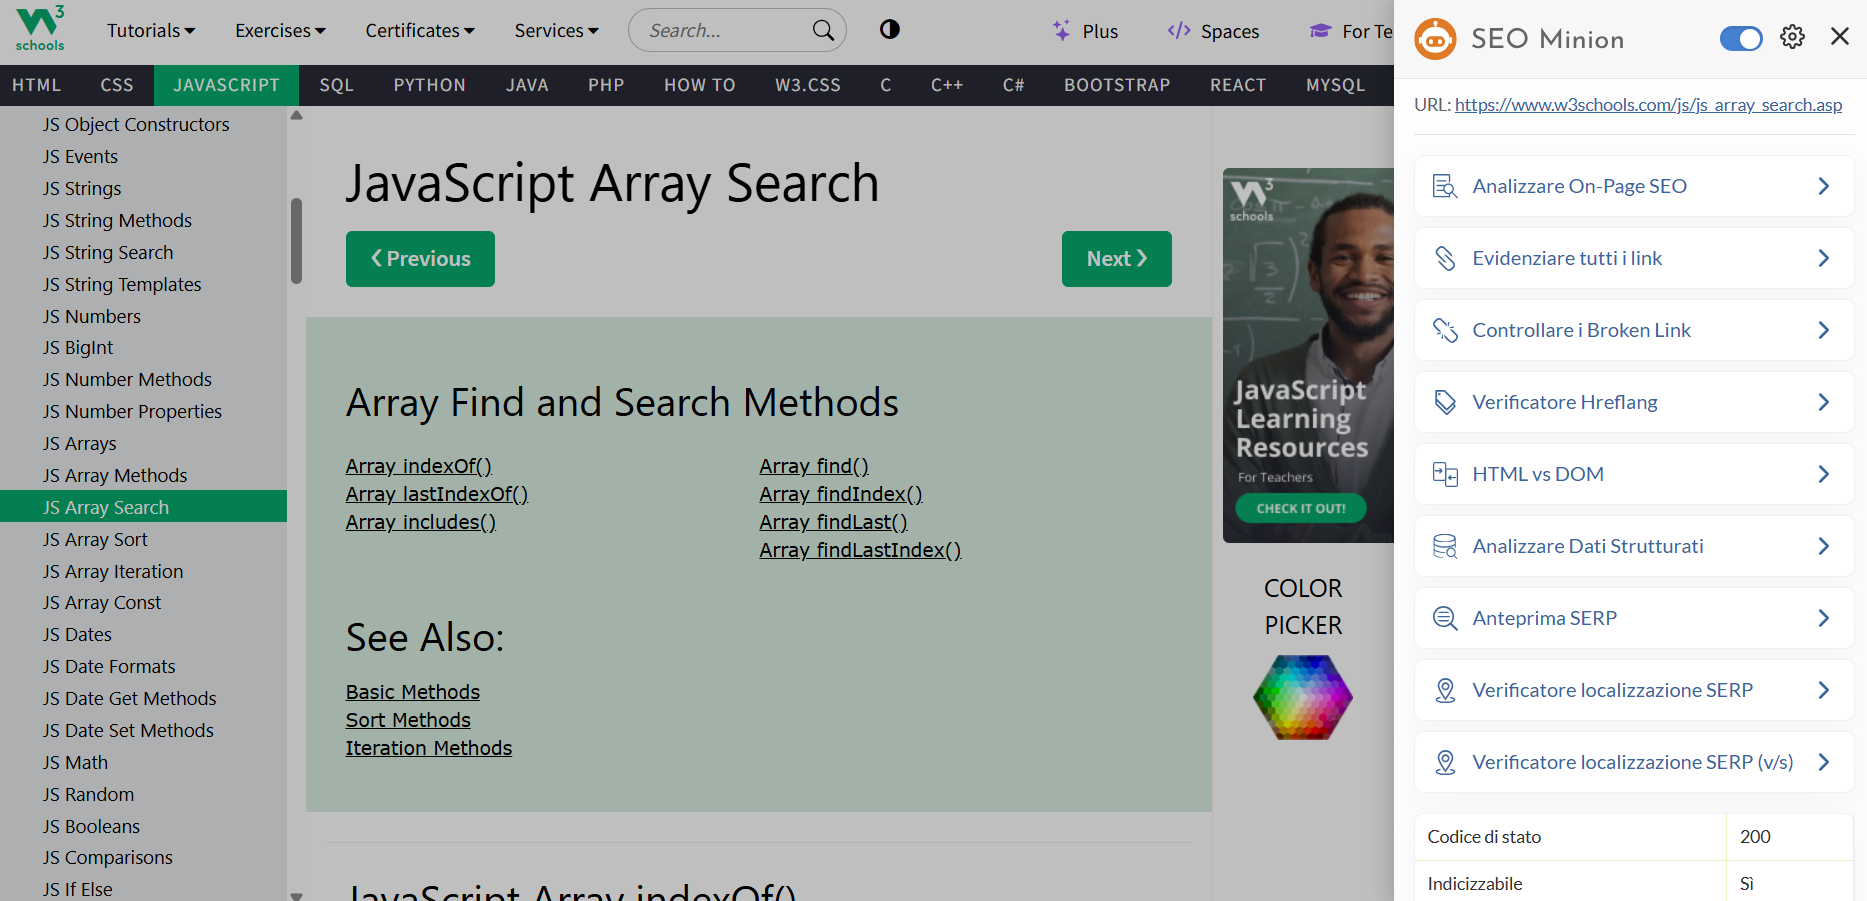
\includegraphics[width=0.9\textwidth]{soluzioni-esistenti/SEO-Minion/seo_minion_sidebar.png} 
    \caption{SEO Minion - sidebar}
\end{figure}

\subsection{Vantaggi}
\par SEO Minion è disponibile come estensione o add-on per Google Chrome, Firefox e Microsoft Edge. Le funzionalità di analisi SEO sono integrate in un'unica piattaforma.

\subsection{Svantaggi}
\par SEO Minion è disponibile solo per i clienti del piano Silver o superiore di Keywords Everywhere.

\begin{figure}[H]
    \centering 
    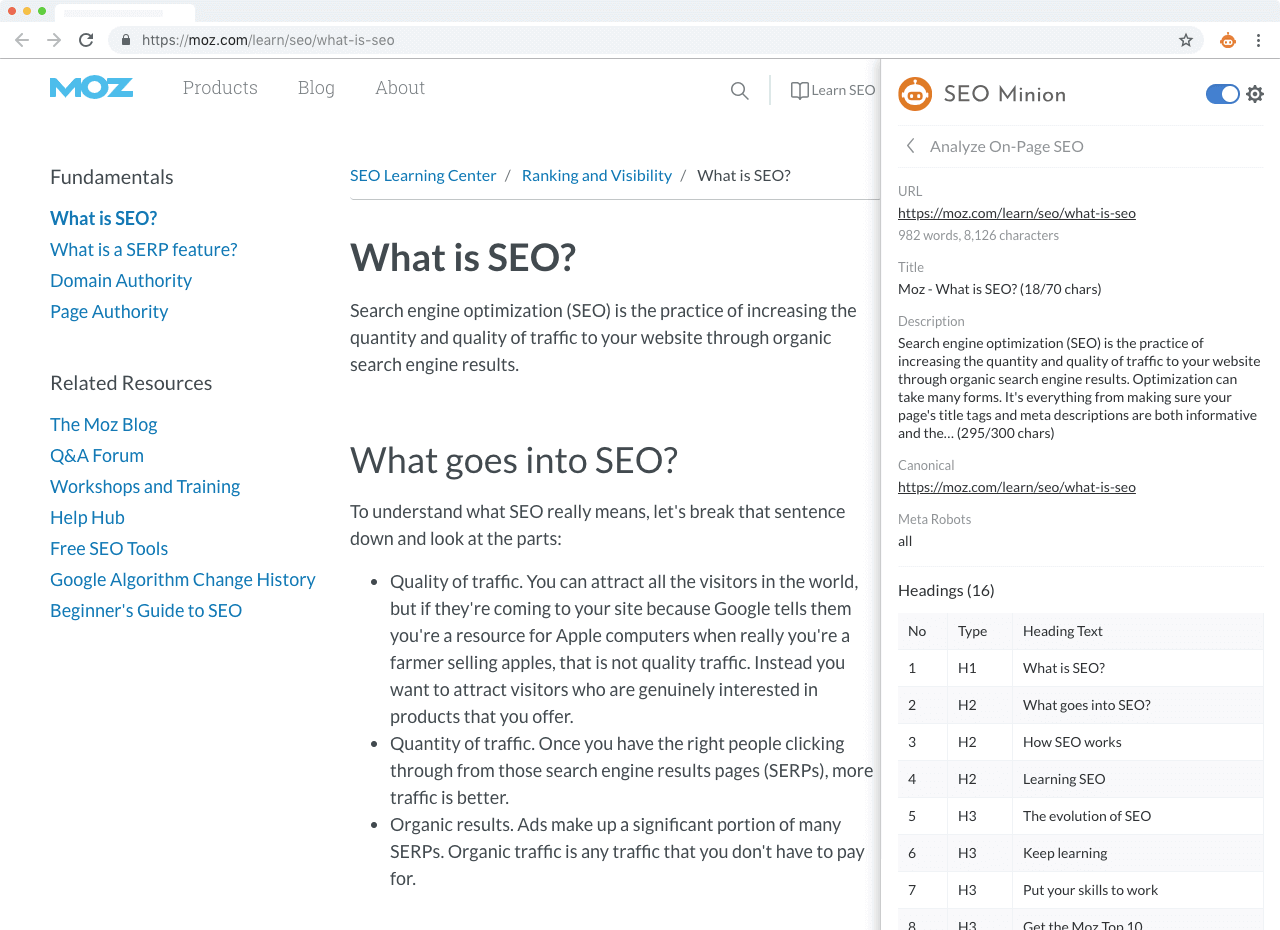
\includegraphics[width=0.8\columnwidth]{soluzioni-esistenti/SEO-Minion/seo_minion_on_page_analysis.png} 
    \caption{SEO Minion - Analisi On-Page}
\end{figure}

\section{SEO Checker}

\subsection{Funzionalità}
\par SEO Checker è uno strumento dell’ecosistema Keywords Everywhere, all’interno del quale troviamo anche il già citato SEO Minion. Mentre quest’ultimo è stato concepito per l’analisi single-page, SEO Checker nasce per superarne i limiti: permette infatti di analizzare siti con migliaia di pagine e integra controlli su velocità e sicurezza.

\begin{figure}[H]
    \centering 
    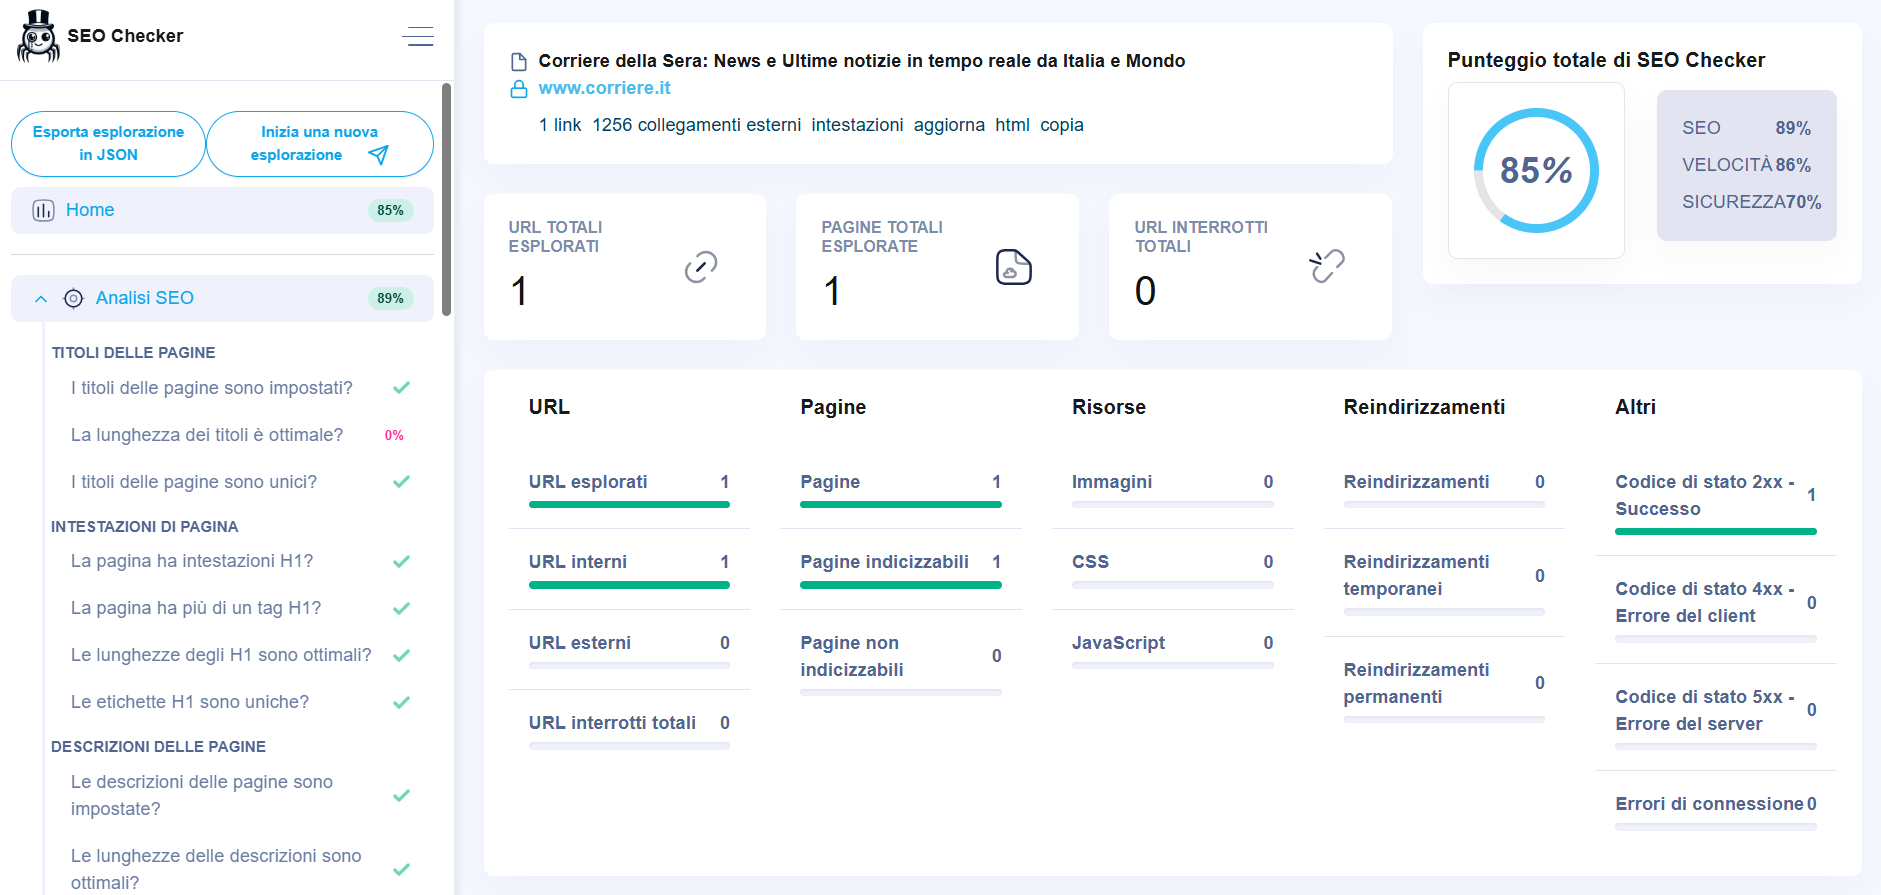
\includegraphics[width=0.8\columnwidth]{soluzioni-esistenti/SEO-Checker/seo_checker_analysis.png} 
    \caption{SEO Checker - Analisi SEO del Corriere della Sera}
\end{figure}

\subsection{Vantaggi}
\par Così come SEO Minion, anche SEO Checker è disponibile come estensione o add-on per Google Chrome, Firefox e Microsoft Edge. Le funzionalità sono integrate in un'unica piattaforma. A differenza di SEO Minion, SEO Checker è disponibile gratuitamente.

\subsection{Svantaggi}
\par SEO Checker fornisce un'analisi dettagliata della SEO on-page, ma risulta carente per quanto riguarda le funzionalità di ricerca e analisi delle parole chiave.

\section{Yoast SEO (plugin per CMS)}

\subsection{Funzionalità}
\par Yoast SEO è un plugin per CMS che semplifica il processo di ottimizzazione SEO. Fornisce feedback in tempo reale per migliorare il posizionamento sui motori di ricerca. La versione del plugin per WordPress consente di ottimizzare le parole chiave (note anche come keyphrase) attraverso un’analisi della densità, della distribuzione e di altri fattori SEO on-page. Con la versione a pagamento, l’utente può anche scegliere delle keyphrase correlate (argomenti collegati o parole chiave secondarie) da valutare distintamente. Inoltre, l’integrazione con Semrush fornisce suggerimenti di keyphrase correlate basati sui volumi di ricerca, sull’intento e sulla keyword difficulty. Naturalmente, i controlli sono meno restrittivi rispetto alla parola chiave principale. Per evitare di dover ripetere meccanicamente la stessa keyphrase, la versione Premium permette anche di aggiungere uno o più sinonimi, che Yoast interpreta allo stesso modo senza penalizzare il punteggio.

\begin{figure}[H]
    \centering 
    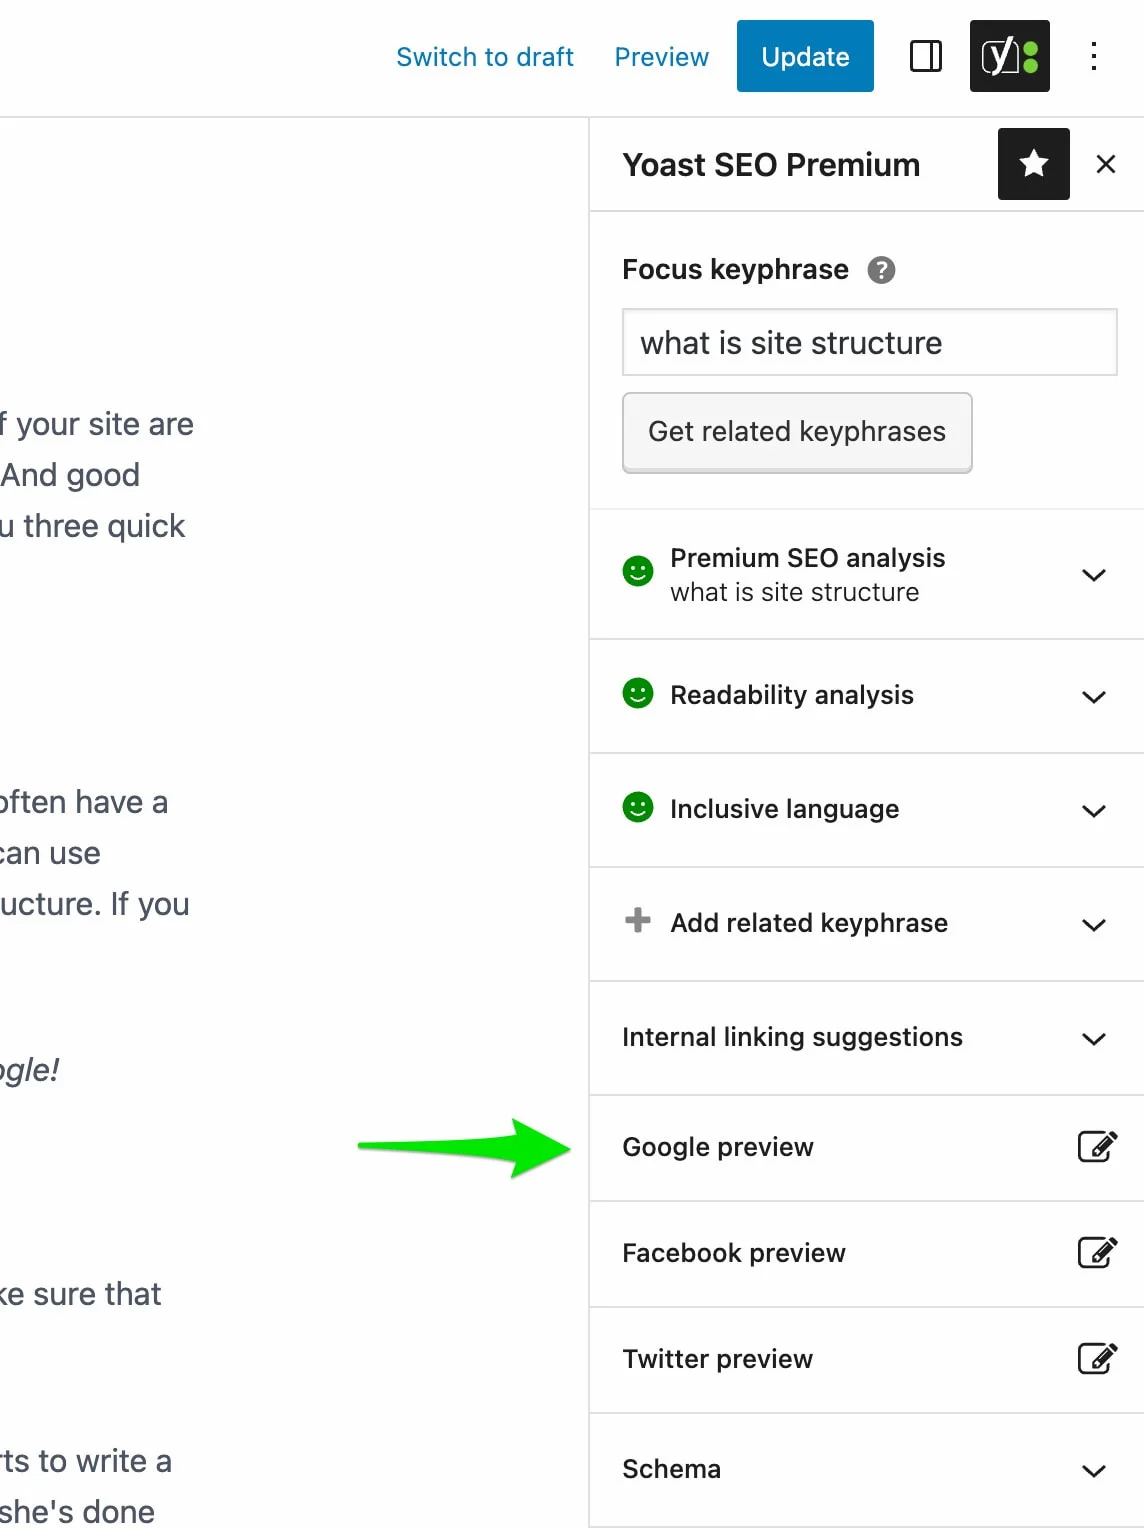
\includegraphics[width=0.4\columnwidth]{soluzioni-esistenti/Yoast-SEO/yoast_seo_sidebar.png} 
    \caption{Yoast SEO - sidebar}
\end{figure}

\subsection{Vantaggi}
\par Yoast SEO è disponibile in versione gratuita per WordPress, seppur con alcune limitazioni, e può essere integrato con altri strumenti SEO come Semrush e Wincher. Il plugin viene aggiornato regolarmente per rimanere allineato agli algoritmi dei motori di ricerca e alle best practice SEO.

\subsection{Svantaggi}
\par Yoast SEO è limitato a CMS come WordPress e Shopify. Alcune funzionalità, tra cui l’inserimento di parole chiave correlate e sinonimi, o l'integrazione con Semrush, richiedono la sottoscrizione di un abbonamento a pagamento.

\begin{figure}[H]
    \centering 
    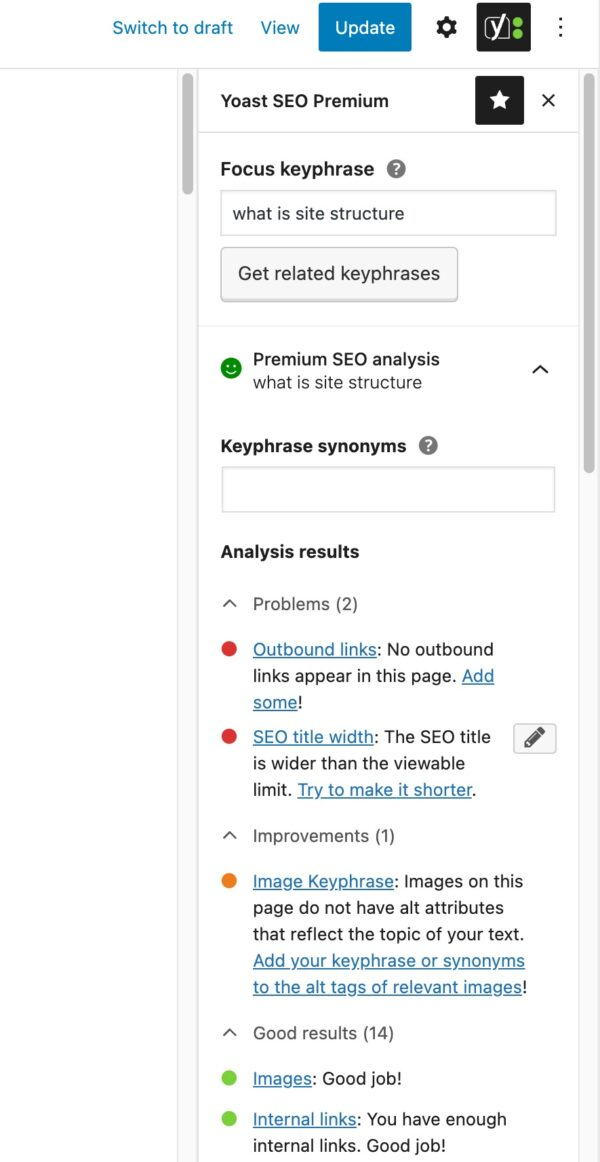
\includegraphics[width=0.4\columnwidth]{soluzioni-esistenti/Yoast-SEO/yoast_seo_premium.png} 
    \caption{Yoast SEO Premium - Analisi SEO}
\end{figure}